\documentclass{article}

\usepackage{microtype}
\usepackage{amsmath}
\usepackage{enumitem}
\usepackage{etoolbox}
% \usepackage[svgnames]{xcolor}
\usepackage{pgfplots, relsize}
\usetikzlibrary{calc}
\usepgfplotslibrary{fillbetween}
\pgfplotsset{compat=newest}

\usepackage{tikz}
\usepackage{tikz-3dplot}
\usepackage[letterpaper, bottom=100pt]{geometry}
\usepackage{physics}
\usepackage{MnSymbol}
\usepackage{float}

\newcommand{\diff}[1]{\frac{#1}{dt}}
\newcommand{\vel}{\mathrm{v}}
\newcommand{\x}{\mathrm{x}}
\newcommand{\inter}{\int_{t_1}^{t_2}}
\newcommand{\tvert}{\biggr\rvert_{t_1}^{t_2}}
\newcommand{\derv}{\frac{\mathrm{d}}{\mathrm{d}t}}

\newcommand{\ddx}{\frac{\mathrm{d}}{\mathrm{d}x}}

\patchcmd\subequations
 {\theparentequation\alph{equation}}
 {\subequationsformat}
 {}{}

\newcommand{\subequationsformat}{\theparentequation.\arabic{equation}}

\author{Laith}
\title{Defining Logarithm as an Integral}
\date{1/30/2023}

\begin{document}
\maketitle

\paragraph{Definition} $\ln(x)$ is a function given by: 
\[\ln(x) = \int_{1}^{x} \frac{1}{t} \,\mathrm{d}t\]
This is true by the \textbf{Fundamental Theorem of Calculus}:
\[\mathrm{F}(x) = \int_{a}^{\mathrm{g}(x)} \mathrm{F}(t)\,\mathrm{d}t 
\,\Rightarrow\, \mathrm{F'}(x) = \mathrm{g'}(x)\cdot\mathrm{F}(\mathrm{g}(x))\]

\section{Discussion}
\begin{center}
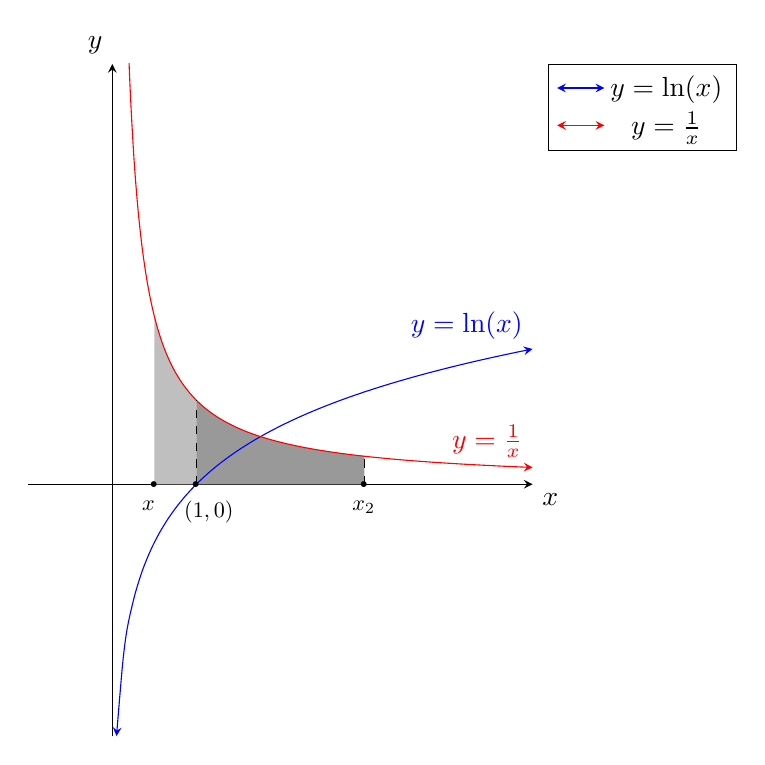
\begin{tikzpicture}
    \begin{axis}
        [
        unit vector ratio* = 2 2 2,
        axis equal image,
        xmin=-1,
        xmax=5,
        ymin=-3, 
        ymax=5, 
        scale=1.5,
        xtick,
        ytick,
        xlabel=$x$,
        ylabel=$y$,
        axis lines=center,
        xlabel style={below right},
        ylabel style={above left},
        smooth,
        legend pos=outer north east,
        smooth,
        no marks,
        samples=100,
        ]
        \path[name path=xAxis] (-1, 0) -- (6, 0);

        \addplot+[name path=A, color=blue, stealth-stealth] {ln(x)} node[above left] {$y=\ln(x)$};
        \addlegendentry[]{$y=\ln(x)$}
        \addplot+[name path=B, color=red, domain=0:5, stealth-stealth] {1/x} node[above left] {$y=\frac{1}{x}$};
        \addlegendentry[]{$y=\frac{1}{x}$}

        \addplot[gray!50] fill between[of=B and xAxis, soft clip={domain=0.5:1}];
        \addplot[gray!80] fill between[of=B and xAxis, soft clip={domain=1:3}];

        \node[scale=2] at (1, 0) {$.$};
        \node[scale=0.8, anchor=north west, xshift=-9, yshift=-4] at (1, 0) {$(1, 0)$};

        \node[scale=2] at (0.5, 0) {$.$};
        \node[scale=0.8, anchor=north west, xshift=-9, yshift=-4] at (0.5, 0) (x) {$x$};

        \draw[dashed] (1, 0) -- (1, 1);

        \node[scale=2] at (3, 0) {$.$};
        \node[scale=0.8, anchor=north west, xshift=-9, yshift=-4] at (3, 0) (x2) {$x_2$};
        \draw[dashed] (3, 0) -- (3, 1/3);

    \end{axis}
\end{tikzpicture}
\end{center}

\begin{align*}
    \text{Case 1}:& \, &0 < x < 1 &; &\ln(x) &= -\int_{x}^{1} \frac{1}{t}\,\mathrm{d}t \\
    \text{Case 2}:& \, &x > 1 &; &\ln(x) &= \int_{1}^{x} \frac{1}{t}\,\mathrm{d}t \\
    \text{Case 2}:& \, &x = 1 &; &\ln(x) &= \int_{1}^{1} \frac{1}{t}\,\mathrm{d}t = 0
\end{align*}

\subsection{Definition:} 
\[\ln(e) = \int_{1}^{e} \frac{1}{t} \mathrm{d}t=1\]

\subsection{Properties of $\ln$:}
If $x>0,\, y>0,\, zy<0$, then:
\begin{enumerate}
    \item $\ln(xy) = \ln(x)+\ln(y)$
    \item $\ln(\frac{x}{y}) = \ln(x)-\ln(y)$
    \item $\ln(x^k) = k\ln(x)$
    \item $\ln(e^x) = x$
\end{enumerate}

\subsection{Derivatives of $y=\ln(x)$ or $y=\ln(\mathrm{u}(x))$:}
\[\ddx[\ln(\mathrm{u}(x))]=\frac{\mathrm{u'}(x)}{\mathrm{u}(x)}\,\,\,\biggr\rvert\,\,\,\ddx[\ln(x)]=\frac{1}{x}\]

\subsection{Integrals:}
\[\int\frac{\mathrm{u'}(x)}{\mathrm{u}(x)}\mathrm{d}x = \ln\left\lvert\mathrm{u}(x)\right\rvert+C\]

\newpage
\section{Examples:}

\end{document}